\chapter{Branch-and-Bound combinatório}
\thispagestyle{empty}

O \textit{Branch-and-Bound} (BB) consiste em um algoritmo de enumeração implícita capaz de resolver problemas combinatórios como o TSP de maneira exata aproveitando-se da noção de \textit{bounds}.

% Relaxações
% - lower bounds
% Limitantes superiores
% Algoritmo branch-and-bound
% BB combinatório para o TSP
% - Assigment problem como uma relaxação para o TSP
% - regra de branching
% diferentes estratégias de busca

% \iffalse
{
% \color{blue}

\section{Relaxações}
Todo problema de otimização combinatória possui um ``espaço de soluções'' associado. Aqui, entende-se por espaço de soluções o conjunto de todas as soluções válidas para uma certa instância do problema. O espaço de soluções para uma instância do TSP envolvendo o conjunto de vértices $\{1,2,\dots,n\}$, por exemplo, é o conjunto de todas as permutações da sequência \((1,2,\dots,n)\). Note que o espaço de soluções de um problema de otimização é diretamente moldado por suas restrições. Quanto mais restrições um problema de otimização combinatória possui, menor tende a ser o número de soluções que são válidas para ele. Em outras palavras, quanto mais restrito um problema de otimização combinatória é, menor é seu espaço de soluções associado. O TSP, por exemplo, possui duas restrições notórias: (\textit{i}) cada uma das $n$ cidades deve ser visitada exatamente uma vez; (\textit{ii}) a sequência de visitas aos vértices deve formar um único \textit{tour} (i.e., deve-se partir de uma cidade e retornar a ela). As figuras \ref{fig:solInvalid1} e \ref{fig:solInvalid2} apresentam soluções que não obedecem às restrições citadas, e que não pertencem ao espaço de soluções da versão original do TSP.
        
% \newsavebox{\tmpboxa}
% \begin{lrbox}{\tmpboxa}
% \begin{dot2tex}[circo]
% graph TSP {
% node [shape=circle, fixedsize = true, width=0.1,style="fill=blue!20"];
% 1;
% 2;
% 3 -- 4;
% 4 -- 5;
% 5 -- 6;
% 6 -- 7;
% 7 -- 3;
% }
% \end{dot2tex}
% \end{lrbox}
% 
% \newsavebox{\tmpboxb}
% \begin{lrbox}{\tmpboxb}
% \begin{dot2tex}[circo]
% graph TSP2 {
% node [shape=circle, fixedsize = true, width=0.1,style="fill=blue!20"];
% 1 -- 2;
% 2 -- 3;
% 3 -- 4;
% 4 -- 1;
% 5 -- 6;
% 6 -- 7;
% 7 -- 5;
% }
% \end{dot2tex}
% \end{lrbox}

\begin{figure}[ht!]
    \centering
    \subfloat[Solução que não obedece à restrição (\textit{i}).]{
        % \includegraphics[width=0.45\textwidth]{example-image-a} 

			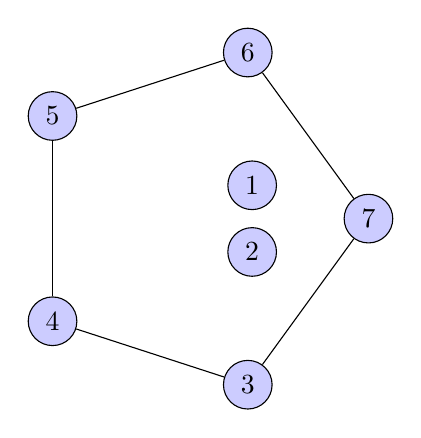
\begin{tikzpicture}[>=latex,line join=bevel,]
				%%
				\node (1) at (75.36bp,75.289bp) [draw,circle,fill=blue!20] {1};
				\node (2) at (75.36bp,51.289bp) [draw,circle,fill=blue!20] {2};
				\node (3) at (73.787bp,3.5bp) [draw,circle,fill=blue!20] {3};
				\node (4) at (3.5bp,26.337bp) [draw,circle,fill=blue!20] {4};
				\node (5) at (3.5bp,100.24bp) [draw,circle,fill=blue!20] {5};
				\node (6) at (73.787bp,123.08bp) [draw,circle,fill=blue!20] {6};
				\node (7) at (117.23bp,63.289bp) [draw,circle,fill=blue!20] {7};
				\draw [] (3) ..controls (58.55bp,8.4506bp) and (19.07bp,21.278bp)  .. (4);
				\draw [] (4) ..controls (3.5bp,42.358bp) and (3.5bp,83.87bp)  .. (5);
				\draw [] (5) ..controls (18.736bp,105.19bp) and (58.217bp,118.02bp)  .. (6);
				\draw [] (6) ..controls (83.203bp,110.12bp) and (107.6bp,76.534bp)  .. (7);
				\draw [] (7) ..controls (107.81bp,50.329bp) and (83.409bp,16.745bp)  .. (3);
				%
			\end{tikzpicture}
			\label{fig:solInvalid1}
		}
		\hspace{0.5cm}
		\subfloat[Solução que não obedece à restrição (\textit{ii}).]{
			% \includegraphics[width=0.45\textwidth]{example-image-a} 
			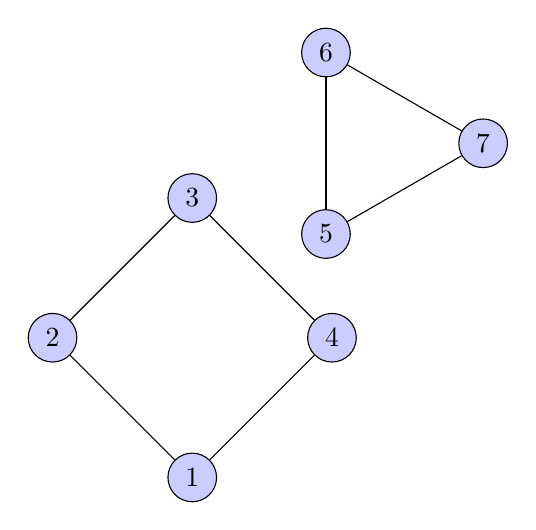
\begin{tikzpicture}[>=latex,line join=bevel,]
				%%
				\node (1) at (53.793bp,3.5bp) [draw,circle,fill=blue!20] {1};
				\node (2) at (3.5bp,53.793bp) [draw,circle,fill=blue!20] {2};
				\node (3) at (53.793bp,104.09bp) [draw,circle,fill=blue!20] {3};
				\node (4) at (104.09bp,53.793bp) [draw,circle,fill=blue!20] {4};
				\node (5) at (101.93bp,91.127bp) [draw,circle,fill=blue!20] {5};
				\node (6) at (101.93bp,156.46bp) [draw,circle,fill=blue!20] {6};
				\node (7) at (158.51bp,123.79bp) [draw,circle,fill=blue!20] {7};
				\draw [] (1) ..controls (42.275bp,15.018bp) and (14.455bp,42.838bp)  .. (2);
				\draw [] (2) ..controls (15.018bp,65.311bp) and (42.838bp,93.131bp)  .. (3);
				\draw [] (3) ..controls (65.311bp,92.568bp) and (93.131bp,64.748bp)  .. (4);
				\draw [] (4) ..controls (92.568bp,42.275bp) and (64.748bp,14.455bp)  .. (1);
				\draw [] (5) ..controls (101.93bp,105.98bp) and (101.93bp,141.56bp)  .. (6);
				\draw [] (6) ..controls (114.8bp,149.03bp) and (145.61bp,131.24bp)  .. (7);
				\draw [] (7) ..controls (145.65bp,116.36bp) and (114.84bp,98.576bp)  .. (5);
				%
			\end{tikzpicture}
			\label{fig:solInvalid2} 
		}
		% \hspace{0.5cm}
		% \subfloat[Solução que não obedece à restrição (\textit{ii}).]{\includegraphics[width=0.45\textwidth]{example-image-b} \label{fig:solInvalid2}}
		% % \includegraphics[width=0.75\textwidth]{example-image-a}
		\caption{Exemplos de soluções inválidas.}
		\label{fig:solucaoExemplosEspaco}
	\end{figure}

Ao retirar uma ou mais restrições de um problema de otimização, obtém-se um novo problema menos restrito. Diz-se que esse novo problema é uma ``relaxação'' do problema original. ``Relaxar'' uma restrição significa, portanto, removê-la do problema. Dito isso, há uma importante relação entre o espaço de soluções de um problema e o de suas relaxações. A Figura \ref{fig:espacoSolucoes}, por exemplo, ilustra o espaço de soluções de diferentes versões do TSP. Observe que o espaço de soluções da versão original do TSP está contido inteiramente no espaço de ambas as relaxações. Essa propriedade é não apenas intuitiva --- soluções para um problema mais restrito não deixam de ser válidas para um problema menos restrito ---, como também é válida para qualquer problema de otimização, e será usada extensivamente nas próximas seções.
 
 \begin{figure}[ht!]
     \centering
     % \includegraphics[width=0.875\textwidth]{example-image-a}
     \begin{tikzpicture}
      \draw[pattern=dots, line width=1pt,  fill=blue!10!red, fill opacity=0.4] plot[smooth cycle] coordinates{ (-2,2) (-3.5,0) (0,-2) (1, 0) };
      \draw[pattern=dots, line width=1pt,  fill=blue, fill opacity=0.3] plot[smooth cycle] coordinates{ (2,2) (3.5,0) (0,-2) (-1, 0) };
      \draw[pattern=dots, line width=0pt] plot[smooth cycle] coordinates{ (-2,2) (-3.5,0) (0,-2) (1, 0) };
      \draw[pattern=dots, line width=0pt] plot[smooth cycle] coordinates{ (2,2) (3.5,0) (0,-2) (-1, 0) };
      
      \node[circle, fill=black, inner sep=0pt, minimum size=4pt] (A) at (2.25,1.5) {};
      \node[] (B) at (3.75,2.35) {Obedece à restrição (\textit{ii})};
      \draw[-, thick] (B) -- (A);
      \node[circle, fill=black, inner sep=0pt, minimum size=4pt] (C) at (-2.25,1.1) {};
      \node[] (D) at (-2.75,2.75) {Obedece à restrição (\textit{i})};
      \draw[-, thick] (D) -- (C);
      \node[circle, fill=black, inner sep=0pt, minimum size=4pt] (E) at (0.25,-1.55) {};
      \node[] (F) at (1,-2.8) {Obedece às restrições (\textit{i}) e (\textit{ii})};
      \draw[-, thick] (F) -- (E);
      
     \end{tikzpicture} 
     \caption{Espaços de soluções de diferentes versões do TSP.}
     \label{fig:espacoSolucoes}
 \end{figure}

% \begin{itemize}
%     \item Figura da Região de soluções de um problema qualquer e região da relaxação (muito maior)
% \end{itemize}

\section{Limitantes}
Considere um problema de minimização qualquer e cuja solução ótima é $s^* \in \mathcal{S}$, em que $\mathcal{S}$ é seu espaço de soluções associado. Analogamente, considere que uma relaxação do mesmo problema está associada a um espaço de soluções $\mathcal{U}$ e uma solução ótima $u^* \in \mathcal{U}$. Já que o segundo problema consiste em uma relaxação do primeiro, então $\mathcal{S} \subseteq \mathcal{U}$, e portanto, a relação $f(u^*) \leq f(s^*)$ é sempre válida. Considere, agora, que $s' \in \mathcal{S}$ é uma solução qualquer --- não necessariamente ótima --- para o primeiro problema.  Já que $s^*$ é a solução ótima, então, por definição, \(f(s^*) \leq f(s')\). Portanto, é garantido que o valor objetivo da solução ótima do primeiro problema se encontra dentro do intervalo $[f(u^*), f(s')]$. Por isso, diz-se que $f(u^*)$ é um limitante inferior (\textit{lower bound}, LB) para o primeiro problema, enquanto $f(s')$ é um limitante superior (\textit{upper bound}, UB).

O conceito de limitantes é útil, por exemplo, para determinar a qualidade de uma solução. Para ver isso, considere que $s'$ é uma solução obtida de maneira heurística e que \[100\% \times \frac{f(s') - f(u^*)}{f(u^*)} \] é a diferença relativa entre $f(s')$ e $f(u^*)$, denominada \textit{gap}. Note que se o \textit{gap} for nulo, então $f(s') = f(u^*)$, o que significa que a solução $s'$ é ótima, já que \[f(u^*) \leq f(s^*) \leq f(s').\] Por isso, quanto mais próximo de zero for o \textit{gap}, maiores são as chances de que $s'$ seja uma solução ótima para o problema. 

O algoritmo \textit{Branch-and-Bound} (BnB), apresentado neste capítulo, se baseia na ideia de diminuir o tamanho do intervalo $[f(u^*), f(s')]$ até que se possa garantir que a solução $s'$ é ótima. O \textit{gap} entre $f(s')$ e $f(u^*)$ funciona, portanto, como um critério de parada para o algoritmo, que finaliza apenas quando ele é nulo.

\section{Algoritmo \textit{Branch-and-Bound}}

O Algoritmo \ref{alg:branchAndBound} descreve o método \textit{Branch-and-Bound} (BnB) para problemas de minimização. Primeiramente, o maior UB encontrado é inicializado com o valor $\infty$ (linha \ref{bnbCriaUBInf}). Após isso, se uma heurística para o problema estiver disponível, ela é usada para gerar um UB válido (linhas \ref{bnbInicioHeuristica}--\ref{bnbInicioHeuristica2}). Em seguida, uma lista de subproblemas $L$ é inicializada com o espaço $\mathcal{U}$, que corresponde ao espaço de soluções associado a uma relaxação qualquer do problema a ser resolvido. Após isso, um subproblema na lista $L$ é escolhido e resolvido (linhas \ref{bnbEscolheSub}--\ref{bnbResolveSub}). Se a solução $s'$ obtida for viável para o problema original, ela passa a ser a melhor solução, e seu valor objetivo passa a ser o menor UB encontrado (linhas \ref{bnbAtualizaUB1}--\ref{bnbAtualizaUB2}). Se, por outro lado, $s'$ não for viável e seu valor objetivo não for maior que o melhor UB, o espaço associado a $U$ é dividido em espaços mais restritos --- e consequentemente menores ---, que são então adicionados a $L$ (linhas \ref{bnbPushL1}--\ref{bnbPushL2}). O procedimento se repete enquanto a lista $L$ não estiver vazia (linha \ref{bnbWhileCondition}).

\begin{algorithm}[ht]
\DontPrintSemicolon
\KwData{..}
\KwResult{$s^*$}
\Begin{
$ \text{UB} \gets \infty$ \; \label{bnbCriaUBInf}
\If{\text{heurística disponível}}{ \label{bnbInicioHeuristica}
Obter solução $s'$ usando heurística \;
$ \text{UB} \gets f(s') $ \;
} \label{bnbInicioHeuristica2}
$L \gets \{\mathcal{U}\}$ \;
\While{$ L \neq \emptyset $}{ \label{bnbWhileCondition}
$ \mathcal{S}' \gets \mathcal{U} \in L $ \; \label{bnbEscolheSub}
$ L \gets L \setminus \mathcal{S}' $ \; 
$s' \gets \text{Resolver}(\mathcal{S}')$ \; \label{bnbResolveSub}
\If{$ s' \text{é viável} $}{ \label{bnbAtualizaUB1}
    \If{$ f(s') < \text{UB} $}{
        $\text{UB} \gets f(s')$ \;
        $s^* \gets s'$ \;
    }
} \label{bnbAtualizaUB2}
\Else{ \label{bnbPushL1}
    \If{$f(s') \leq \text{UB}$} {
    Dividir $\mathcal{S}'$ em subproblemas mais restritos $\mathcal{S}_1,\mathcal{S}_2,\dots,\mathcal{S}_k$  \;
$L \gets L \cup \{\mathcal{S}_1, \mathcal{S}_2, \dots, \mathcal{S}_k\}$ \;
    } \label{bnbPushL2}
}
}

\Return $s^*$ \;
}
\caption{\textsc{Branch-and-Bound}\label{alg:branchAndBound}}
\end{algorithm}

Para compreender a ideia geral por trás do Algoritmo \ref{alg:branchAndBound}, observe a Figura \ref{alg:branchAndBound}, que mostra o processo de subdivisão da região de soluções da relaxação de um problema de otimização qualquer. O espaço de soluções associados ao problema original e uma relaxação são representados por um círculo tracejado e uma região oval, respectivamente, na Figura \ref{fig:exBnBReg1}. Inicialmente, um LB foi obtido resolvendo-se a relaxação do problema na otimalidade, e apresenta o valor $f(u^*)$. Além disso, uma solução $s'$ para o problema foi obtida de forma heurística, e possui um valor objetivo $f(s') = 110$. Nesse momento, a solução ótima do problema original ($ s^* $) é desconhecida. 

\begin{figure}[ht!]
    \centering
    \subfloat[Primeira iteração]{
        % \includegraphics[width=0.45\textwidth]{example-image-a} 
        \scalebox{0.45}
        {
        \begin{tikzpicture}
        \draw[line width = 1pt, fill=gray!30] (0,0) circle [x radius=5cm, y radius=3.5cm, rotate=30];
        \draw[line width = 1pt, fill=gray!30, dashed] (-0.5,-0.5) circle [radius=2.5cm];
        
        \draw[line width = 0pt, pattern=dots] (0,0) circle [x radius=5cm, y radius=3.5cm, rotate=30];
        % \draw[pattern=dots, line width=0pt] plot[smooth cycle] coordinates{ (-2,2) (-3.5,0) (0,-2) (1, 0) };
        % \draw[pattern=dots, line width=0pt] plot[smooth cycle] coordinates{ (2,2) (3.5,0) (0,-2) (-1, 0) };
        \node[circle, fill=black, inner sep=0pt, minimum size=6pt] (C) at (-0.75,2.95) {};
        \node[] (D) at (-1.5,4.75) {\Huge $u^*$};
        \draw[-, thick] (D) -- (C);
        
        \node[circle, fill=black, inner sep=0pt, minimum size=6pt] (A) at (1.1,0.8) {};
        \node[] (B) at (5.5,2.8) {\Huge $s'$};
        \draw[-, thick] (B) -- (A);
        
        \node[circle, fill=black, inner sep=0pt, minimum size=6pt] (U) at (-2,0) {};
        \node[] (V) at (-5.5,1.25) {\huge $s^*$};
        \draw[-, thick] (U) -- (V);
        
        \node[yshift = -0.875cm, rectangle, draw=black, line width = 1pt, inner sep = 10pt, rounded corners = 0.25cm] at (current bounding box.south) {\Huge $f(u^*) = 90$, $f(s') = 110$};
        \end{tikzpicture}
        }
        \label{fig:exBnBReg1} 
    }
    \hspace{1cm}
    \subfloat[Segunda iteração]{
        % \includegraphics[width=0.45\textwidth]{example-image-a} 
        \scalebox{0.45}
        {
        \begin{tikzpicture}
        \draw[line width = 1pt, pattern=dots, fill=gray!30, dashed, opacity = 0.325] (0,0) circle [x radius=5cm, y radius=3.5cm, rotate=30];
        
        \draw[pattern=dots, line width=1pt, fill=gray!70, fill opacity=0.5] plot[smooth cycle] coordinates{ (-4, -2) (-0.5, -3) (-1.5, 2.5) };
        \draw[pattern=dots, line width=1pt, fill=gray!70, fill opacity=0.5] plot[smooth cycle] coordinates{ (4, 2) (0, 3) (1, -2.75) };
        
        \fill[line width = 0pt, pattern=dots] (0,0) circle [x radius=5cm, y radius=3.5cm, rotate=30];
        % \draw[pattern=dots, line width=0pt] plot[smooth cycle] coordinates{ (-2,2) (-3.5,0) (0,-2) (1, 0) };
        % \draw[pattern=dots, line width=0pt] plot[smooth cycle] coordinates{ (2,2) (3.5,0) (0,-2) (-1, 0) };
        \node[circle, fill=black, inner sep=0pt, minimum size=6pt] (C) at (-0.75,2.95) {};
        \node[] (D) at (-1.5,4.75) {\Huge $u^*$};
        \draw[-, thick] (D) -- (C);
        
        \node[circle, fill=black, inner sep=0pt, minimum size=6pt] (J) at (-3.27,-0.75) {};
        \node[] (K) at (-5.65,0.45) {\huge $u^*_1$};
        \draw[-, thick] (J) -- (K);
        
        \node[circle, fill=black, inner sep=0pt, minimum size=6pt] (I) at (3,2) {};
        \node[] (J) at (5.5,0.15) {\Huge $u^*_2$};
        \draw[-, thick] (I) -- (J);
        
        \node[yshift = -0.875cm, rectangle, draw=black, line width = 1pt, inner sep = 10pt, rounded corners = 0.25cm] at (current bounding box.south) {\Huge $f(u_1^*) = 95$, $f(u_2^*) = 115$};
        
        \draw[line width = 1pt, fill=blue!30, fill opacity = 0.0, dashed] (-0.5,-0.5) circle [radius=2.5];
        
        \end{tikzpicture}
        }
        \label{fig:exBnBReg2} 
    }
    
    \subfloat[Terceira iteração]{
        % \includegraphics[width=0.45\textwidth]{example-image-a} 
        \scalebox{0.45}
        {
        \begin{tikzpicture}
        \draw[line width = 1pt, pattern=dots, fill=gray!30, dashed, opacity = 0.325] (0,0) circle [x radius=5cm, y radius=3.5cm, rotate=30];
        
        
        \draw[pattern=dots, line width=1pt, fill=gray!70, fill opacity=0.5, opacity = 0.25, dashed] plot[smooth cycle] coordinates{ (-4, -2) (-0.5, -3) (-1.5, 2.5) };
        \draw[pattern=dots, line width=1pt, fill=gray!70, fill opacity=0.5, opacity = 0.25, dashed] plot[smooth cycle] coordinates{ (4, 2) (0, 3) (1, -2.75) };
        
        \draw[pattern=dots, line width=1pt, fill=gray!70, fill opacity=0.5] plot[smooth cycle] coordinates{ (-3.785, -1.95) (-0.85, -3) (-1, -2) (-2.7, -1.05) };
        \draw[pattern=dots, line width=1pt, fill=gray!70, fill opacity=0.5] plot[smooth cycle] coordinates{ (-3.0, -0.15) (-0.85, -1.6) (-1.5, 1.9) };
        
        \fill[line width = 0pt, pattern=dots] (0,0) circle [x radius=5cm, y radius=3.5cm, rotate=30];
        % \draw[pattern=dots, line width=0pt] plot[smooth cycle] coordinates{ (-2,2) (-3.5,0) (0,-2) (1, 0) };
        % \draw[pattern=dots, line width=0pt] plot[smooth cycle] coordinates{ (2,2) (3.5,0) (0,-2) (-1, 0) };
        \node[circle, fill=black, inner sep=0pt, minimum size=6pt] (J) at (-3.27,-0.75) {};
        \node[] (K) at (-5.65,0.45) {\huge $u^*_1$};
        \draw[-, thick] (J) -- (K);
        
        \node[circle, fill=black, inner sep=0pt, minimum size=6pt] (Y) at (-3.545,-1.9) {};
        \node[] (Z) at (-5.55,-2.75) {\huge $u^*_3$};
        \draw[-, thick] (Y) -- (Z);
        
        \node[circle, fill=black, inner sep=0pt, minimum size=6pt] (U) at (-2,0) {};
        \node[] (V) at (-4,2.85) {\huge $u^*_4$};
        \draw[-, thick] (U) -- (V);
        
        \draw[line width = 1pt, fill=blue!30, fill opacity = 0.0, dashed] (-0.5,-0.5) circle [radius=2.5];
        
        \node[yshift = -0.875cm, rectangle, draw=black, line width = 1pt, inner sep = 10pt, rounded corners = 0.25cm] at (current bounding box.south) {\Huge $f(u_3^*) = 112$, $f(u_4^*) = 105$};
        
        \end{tikzpicture}
        }
        \label{fig:exBnBReg3} 
    }
    
    \caption{Exemplo ilustrativo de algumas das iterações do BnB.}
    \label{fig:exBnBRegioes}
\end{figure}


Suponha, agora, que fôssemos capazes de dividir a região associada à relaxação do problema em duas novas regiões mais restritas que excluem a solução $u^*$. O processo, chamado de \textit{branching}, é mostrado na Figura \ref{fig:exBnBReg2}, e deve ser feito de forma que a solução $s^*$ ainda esteja dentro de ao menos uma das regiões resultantes. Novamente, os problemas associados às regiões resultantes são resolvidos na otimalidade, gerando as soluções inviáveis $u^*_1$ e $u^*_2$. Note, no entanto, que a solução $u^*_2$ possui um valor objetivo maior que o da melhor solução viável encontrada $(s')$. Portanto, o espaço da direita pode ser ignorado, e precisa-se explorar apenas a região associada à solução $u^*_1$.

Na terceira iteração, mostrada na Figura \ref{fig:exBnBReg3}, a região esquerda é dividida em duas novas regiões que excluem a solução $u^*_1$. Novamente, a solução $u^*_3$ possui um valor objetivo maior que o melhor UB conhecido, e sua região pode ser ignorada. A solução $u^*_4$, por sua vez, é viável para o problema original, e possui um valor objetivo menor que o de $s'$, passando a ser o novo melhor UB encontrado. Observe, ainda, que não faz sentido dividir a região associada à solução $u^*_4$ em regiões menores. Fazer isso apenas geraria soluções cujo valor objetivo é maior ou igual ao atual melhor UB $f(u^*_4)$. Assim, já que não há mais nenhuma região a ser explorada, a solução $u_4^*$ é a solução ótima para o problema.


Em suma, o BnB consiste em uma maneira inteligente de enumerar os elementos do espaço de soluções de um problema de otimização combinatória. O método é genérico, servindo como base para todos os algoritmos exatos apresentados no restante deste livro. Também é importante destacar o impacto positivo que o UB inicial $f(s')$ teve no exemplo mostrado. Se uma heurística não estivesse inicialmente disponível, e consequentemente o UB $f(s')$ não fosse conhecido, não teria sido possível ignorar a região associada à solução $u^*_2$. Consequentemente, determinar a solução ótima para o problema poderia exigir muito mais iterações. Por esse motivo, a elaboração de boas heurísticas é crucial para o bom desempenho dos algoritmos exatos. 


% A ideia do Algoritmo \ref{alg:branchAndBound} é começar em uma relaxação do problema original. Então, o espaço de soluções associado a essa relaxação é subdividido em espaços cada vez menores, associados a versões mais restritas dessa relaxação. Essa etapa é conhecida como \textit{branching}, e deve ser executada de tal forma que saiba-se, com certeza, que a solução ótima reside em algum dos espaços de soluções na lista $L$. Além disso, o algoritmo aproveita-se dos limitantes (\textit{bounds}) para evitar resolver subproblemas de forma desnecessária: se a solução ótima de um problema tiver um valor objetivo maior que o melhor UB, não faz sentido explorar a região associada a ele. Portanto, o BnB nada mais é que uma maneira mais inteligente de enumerar as soluções de um problema. Além disso, o método é genérico e serve como base para os algoritmos dos próximos capítulos.


% \begin{itemize}
%     \item Figura de Árvore do BnB com alguns nós e \textit{bounds}
% \end{itemize}

\section{Branch-and-bound para o TSP}

Para aplicar o BnB a um problema de otimização combinatória, é necessário definir uma relaxação para o problema e um método de \textit{branching}. Neste capítulo, será utilizado o \textit{Assignment Problem} (AP), que é um problema de otimização combinatória que, se parametrizado de maneira apropriada, pode ser interpretado como uma relaxação para o TSP. 

Tanto o AP quanto o método de \textit{branching} necessários para aplicar o BnB ao TSP serão definidos nas próximas seções.

\subsection{Transformação do TSP em um AP}

Sejam $U$ um conjunto de trabalhadores e $W$ um conjunto de tarefas em que $|U| = |W|$. Designar um trabalhador $i \in U$ a uma tarefa $j \in W$ incorre um custo $w_{ij}$. O AP visa designar cada trabalhador a exatamente uma tarefa e cada tarefa a exatamente um trabalhador de forma que a soma total dos custos seja mínima. A Figura \ref{fig:assignExample1} mostra uma solução para uma instância do AP em que $U = \{1,2,\dots,5\}$ e $W = \{6,7,\dots,10\}$. O custo da solução é 
\[
	w_{17} + w_{36} + w_{29} + w_{58} + w_{4,10}.
\]

\begin{figure}[ht]

\centering
\begin{tikzpicture}

\draw[rounded corners = 0.25cm, pattern = dots, dashed, opacity=0.35] (-0.65, 0.65) rectangle (0.65, -0.65 -4 * 1.25);
\draw[rounded corners = 0.25cm, pattern = dots, dashed, opacity=0.35] (-0.65 + 3.5, 0.65) rectangle (0.65 + 3.5, -0.65 -4 * 1.25);
\node[] at (0,1) {$U$};
\node[] at (3.5,1) {$W$};

\node[circle, draw=black, fill=white, line width = 0.05cm] (1)  at (0,0)        {1 };
\node[circle, draw=black, fill=white, line width = 0.05cm] (2)  at (0,-1 * 1.25) {2 };
\node[circle, draw=black, fill=white, line width = 0.05cm] (3)  at (0,-2 * 1.25) {3 };
\node[circle, draw=black, fill=white, line width = 0.05cm] (4)  at (0,-3 * 1.25) {4 };
\node[circle, draw=black, fill=white, line width = 0.05cm] (5)  at (0,-4 * 1.25) {5 };

\node[circle, draw=black, fill=black, text=white] (6)  at (3.5,0)        {6 };
\node[circle, draw=black, fill=black, text=white] (7)  at (3.5,-1 * 1.25) {7 };
\node[circle, draw=black, fill=black, text=white] (8)  at (3.5,-2 * 1.25) {8 };
\node[circle, draw=black, fill=black, text=white] (9)  at (3.5,-3 * 1.25) {9 };
\node[circle, draw=black, fill=black, text=white] (10) at (3.5,-4 * 1.25) {10};

\draw[-{latex}, line width = 0.04cm, color=black] (1) -- node[pos = 0.325, circle, fill=white, inner sep = 1pt] {$w_{17}$} (7);
\draw[-{latex}, line width = 0.04cm, color=black] (2) -- node[pos = 0.5, circle, fill=white, inner sep = 1pt]   {$w_{29}$} (9);
\draw[-{latex}, line width = 0.04cm, color=black] (3) -- node[pos = 0.45, circle, fill=white, inner sep = 1pt]  {$w_{36}$} (6);
\draw[-{latex}, line width = 0.04cm, color=black] (4) -- node[pos = 0.625, circle, fill=white, inner sep = 1pt] {$w_{4,10}$} (10);
\draw[-{latex}, line width = 0.04cm, color=black] (5) -- node[pos = 0.525, circle, fill=white, inner sep = 1pt] {$w_{58}$} (8);

\end{tikzpicture}
\caption{Exemplo de solução para uma instância do AP}\label{fig:assignExample1}

\end{figure}

Para entender como o AP pode ser visto como uma relaxação do TSP, é necessário desenvolver um método que seja capaz de transformar uma instância arbitrária do TSP em um instância do AP. Considere, então, que o grafo completo $G = (V,E)$, em que $V=\{1,2,\dots,n\}$, é uma instância qualquer do TSP. A instância do AP deve ser construída fazendo-se $U = V = W$ e 
\begin{align*}
w_{ij} = \begin{cases}
	c_{ij} & \text{ se } i \neq j \\
	\infty & \text{ se } i = j
\end{cases}
\end{align*}
para todo $i \in U$, $j \in W$\footnote{Devido à natureza do AP, a transformação obriga cada nó a se conectar a algum outro nó. Fazer $w_{ij} = \infty$ para todo $i \in U$, $j \in W$, $i = j$ impede  que um nó seja conectado a ele mesmo, já que o problema é de minimização.}. O resultado da transformação descrita é uma instância específica do AP que possui uma correspondência com a instância do TSP que a originou. Esse problema de otimização combinatória --- que consiste em uma versão especial do AP --- será chamado, daqui em diante, de $\text{AP}_{\text{TSP}}$.

A ligação entre o TSP e o $\text{AP}_{\text{TSP}}$ pode ser compreendida observando-se as figuras \ref{fig:transTSPAP1} e \ref{fig:transTSPAP2}, que mostram duas soluções para uma instância do $\text{AP}_{\text{TSP}}$. As figuras \ref{fig:transTSPAP3} e \ref{fig:transTSPAP4} mostram uma representação alternativa das soluções das figuras \ref{fig:transTSPAP1} e \ref{fig:transTSPAP2}, respectivamente. É interessante notar que embora ambas as soluções sejam válidas para o $\text{AP}_{\text{TSP}}$, apenas a primeira delas é viável para o TSP. É fácil perceber, na verdade, que qualquer solução viável para o TSP também é viável para o $\text{AP}_{\text{TSP}}$. Por isso, o $\text{AP}_\text{TSP}$ é uma relaxação do TSP.

A vantagem de usar o $\text{AP}_{\text{TSP}}$ como relaxação para o TSP é que existem algoritmos que resolvem o AP em tempo polinomial. Um deles é o Algoritmo Húngaro, que é capaz de resolver o AP em tempo $\mathcal{O}(n^3)$, em que $n = |U| = |W|$. Uma implementação do Algoritmo Húngaro e do método de transformação do TSP no $\text{AP}_{\text{TSP}}$, acompanhada de um leitor de instâncias do TSP, pode ser obtida no seguinte \textit{link}: \url{https://github.com/carlosvinicius01/kit-opt/tree/master/BB-Combinat%C3%B3rio/algoritmo-hungaro}. 


% \newsavebox{\tmpboxc}
% \begin{lrbox}{\tmpboxc}
% \begin{dot2tex}[circo]
% digraph TSP {
% node [shape=circle, fixedsize = true, width=0.1,style="fill=white!20"];
% edge [style="-triangle 45"];
% 1 -> 2;
% 2 -> 4;
% 3 -> 1;
% 4 -> 5;
% 5 -> 3;
% }
% \end{dot2tex}
% \end{lrbox}
% 
% \newsavebox{\tmpboxd}
% \begin{lrbox}{\tmpboxd}
% \begin{dot2tex}[circo]
% digraph TSP {
% node [shape=circle, fixedsize = true, width=0.1,style="fill=white!20"];
% edge [style="-triangle 45"];
% 1 -> 2;
% 2 -> 4;
% 3 -> 5;
% 4 -> 1;
% 5 -> 3;
% }
% \end{dot2tex}
% \end{lrbox}

\begin{figure}[htpb!]
	\centering
    \subfloat[Solução para o $\text{AP}_{\text{TSP}}$]
		{
        \scalebox{0.9}
        {
        	\begin{tikzpicture}

						\draw[rounded corners = 0.25cm, pattern = dots, dashed, opacity=0.35] (-0.65, 0.65) rectangle (0.65, -0.65 -4 * 1.00);
						\draw[rounded corners = 0.25cm, pattern = dots, dashed, opacity=0.35] (-0.65 + 3.5, 0.65) rectangle (0.65 + 3.5, -0.65 -4 * 1.00);
						\node[] at (0,1) {$U$};
						\node[] at (3.5,1) {$W$};

						\node[circle, draw=black, fill=white, line width = 0.05cm] (1)  at (0,0)        {1 };
						\node[circle, draw=black, fill=white, line width = 0.05cm] (2)  at (0,-1 * 1.0) {2 };
						\node[circle, draw=black, fill=white, line width = 0.05cm] (3)  at (0,-2 * 1.0) {3 };
						\node[circle, draw=black, fill=white, line width = 0.05cm] (4)  at (0,-3 * 1.0) {4 };
						\node[circle, draw=black, fill=white, line width = 0.05cm] (5)  at (0,-4 * 1.0) {5 };

						\node[circle, draw=black, fill=black, text=white] (6)  at (3.5,0)        {1};
						\node[circle, draw=black, fill=black, text=white] (7)  at (3.5,-1 * 1.0) {2};
						\node[circle, draw=black, fill=black, text=white] (8)  at (3.5,-2 * 1.0) {3};
						\node[circle, draw=black, fill=black, text=white] (9)  at (3.5,-3 * 1.0) {4};
						\node[circle, draw=black, fill=black, text=white] (10) at (3.5,-4 * 1.0) {5};

						\draw[-{latex}, line width = 0.04cm, color=black] (1) -- (7);
						\draw[-{latex}, line width = 0.04cm, color=black] (2) -- (9);
						\draw[-{latex}, line width = 0.04cm, color=black] (3) -- (6);
						\draw[-{latex}, line width = 0.04cm, color=black] (4) -- (10);
						\draw[-{latex}, line width = 0.04cm, color=black] (5) -- (8);

        	\end{tikzpicture}
        }
        \label{fig:transTSPAP1} 
    }
		\hspace{0.1cm}
    \subfloat[Solução para o $\text{AP}_{\text{TSP}}$]
		{
        \scalebox{0.9}
        {
        	\begin{tikzpicture}

						\draw[rounded corners = 0.25cm, pattern = dots, dashed, opacity=0.35] (-0.65, 0.65) rectangle (0.65, -0.65 -4 * 1.00);
						\draw[rounded corners = 0.25cm, pattern = dots, dashed, opacity=0.35] (-0.65 + 3.5, 0.65) rectangle (0.65 + 3.5, -0.65 -4 * 1.00);
						\node[] at (0,1) {$U$};
						\node[] at (3.5,1) {$W$};

						\node[circle, draw=black, fill=white, line width = 0.05cm] (1)  at (0,0)        {1 };
						\node[circle, draw=black, fill=white, line width = 0.05cm] (2)  at (0,-1 * 1.0) {2 };
						\node[circle, draw=black, fill=white, line width = 0.05cm] (3)  at (0,-2 * 1.0) {3 };
						\node[circle, draw=black, fill=white, line width = 0.05cm] (4)  at (0,-3 * 1.0) {4 };
						\node[circle, draw=black, fill=white, line width = 0.05cm] (5)  at (0,-4 * 1.0) {5 };

						\node[circle, draw=black, fill=black, text=white] (6)  at (3.5,0)        {1};
						\node[circle, draw=black, fill=black, text=white] (7)  at (3.5,-1 * 1.0) {2};
						\node[circle, draw=black, fill=black, text=white] (8)  at (3.5,-2 * 1.0) {3};
						\node[circle, draw=black, fill=black, text=white] (9)  at (3.5,-3 * 1.0) {4};
						\node[circle, draw=black, fill=black, text=white] (10) at (3.5,-4 * 1.0) {5};

						\draw[-{latex}, line width = 0.04cm, color=black] (1) -- (7);
						\draw[-{latex}, line width = 0.04cm, color=black] (2) -- (9);
						\draw[-{latex}, line width = 0.04cm, color=black] (3) -- (10);
						\draw[-{latex}, line width = 0.04cm, color=black] (4) -- (6);
						\draw[-{latex}, line width = 0.04cm, color=black] (5) -- (8);

        	\end{tikzpicture}
        }
        \label{fig:transTSPAP2} 
    }
		\vfill
		\vspace{0.5cm}
		\subfloat[Solução viável para o TSP]
		{
			\scalebox{0.9}
			{
				\begin{tikzpicture}[>=latex,line join=bevel,]
					%%
					\node (1) at (73.787bp,3.5bp) [draw,circle,fill=white!20] {1};
					\node (2) at (3.5bp,26.337bp) [draw,circle,fill=white!20] {2};
					\node (4) at (3.5bp,100.24bp) [draw,circle,fill=white!20] {4};
					\node (5) at (73.787bp,123.08bp) [draw,circle,fill=white!20] {5};
					\node (3) at (117.23bp,63.289bp) [draw,circle,fill=white!20] {3};
					\draw [->,-triangle 45] (1) ..controls (60.864bp,7.6988bp) and (33.438bp,16.61bp)  .. (2);
					\draw [->,-triangle 45] (2) ..controls (3.5bp,39.974bp) and (3.5bp,69.043bp)  .. (4);
					\draw [->,-triangle 45] (4) ..controls (16.423bp,104.44bp) and (43.849bp,113.35bp)  .. (5);
					\draw [->,-triangle 45] (3) ..controls (109.24bp,52.297bp) and (92.289bp,28.967bp)  .. (1);
					\draw [->,-triangle 45] (5) ..controls (81.773bp,112.09bp) and (98.723bp,88.756bp)  .. (3);
					%
				\end{tikzpicture}
			}
			\label{fig:transTSPAP3}
		}
		\hspace{0.1cm}
		\subfloat[Solução inviável para o TSP]
		{
			\scalebox{0.9}
			{
				\begin{tikzpicture}[>=latex,line join=bevel,]
					%%
					\node (1) at (3.5bp,3.5bp) [draw,circle,fill=white!20] {1};
					\node (2) at (3.5bp,68.832bp) [draw,circle,fill=white!20] {2};
					\node (4) at (60.08bp,36.166bp) [draw,circle,fill=white!20] {4};
					\node (3) at (66.86bp,66.166bp) [draw,circle,fill=white!20] {3};
					\node (5) at (145.86bp,66.166bp) [draw,circle,fill=white!20] {5};
					\draw [->,-triangle 45] (1) ..controls (3.5bp,15.875bp) and (3.5bp,39.528bp)  .. (2);
					\draw [->,-triangle 45] (2) ..controls (14.217bp,62.645bp) and (34.702bp,50.818bp)  .. (4);
					\draw [->,-triangle 45] (4) ..controls (49.363bp,29.979bp) and (28.878bp,18.152bp)  .. (1);
					\draw [->,-triangle 45] (3) ..controls (79.327bp,73.291bp) and (114.39bp,74.108bp)  .. (5);
					\draw [->,-triangle 45] (5) ..controls (133.39bp,59.041bp) and (98.331bp,58.224bp)  .. (3);
					%
				\end{tikzpicture}
			}
			\label{fig:transTSPAP4}
		}
		\caption{Soluções do $\text{AP}_{\text{TSP}}$}\label{fig:transTSPAP}
\end{figure}

% \begin{itemize}
%     \item Figura de instância e solução do Assignment lado a lado (grafo bipartido)
%     \item Figura de transformação do TSP em assigment (exemplos de solução viavel e inviavel)
% \end{itemize}
\subsection{Regra de \textit{branching}}

Suponha que uma instância do TSP foi convertida em uma instância do $\text{AP}_{\text{TSP}}$, que foi então resolvida por meio do Algoritmo Húngaro. Sabe-se que se a solução obtida for viável para o TSP, ela é a solução ótima. Caso contrário, é necessário dividir a região de soluções em regiões diferentes, de forma que a solução obtida não esteja contida em nenhuma das regiões resultantes. Uma forma simples de garantir isso é escolher o menor \textit{subtour} da solução e proibir cada um de seus arcos separadamente, conforme mostrado na Figura \ref{fig:exemploArvore}. Na figura, inicia-se com uma solução para o $\text{AP}_{\text{TSP}}$, que é inviável para o TSP por possuir dois \textit{subtours}. Nesse caso, o menor \textit{subtour} é aquele que contém os nós 3 e 5. Então, duas novas instâncias do $\text{AP}_{\text{TSP}}$ são geradas: a primeira delas proíbe o arco $(5,3)$, enquanto a segunda proíbe o arco $(3,5)$. Um arco $a$ pode ser proibido fazendo-se $c_a = \infty$.

% \newsavebox{\tmpboxe}
% \begin{lrbox}{\tmpboxe}
% \begin{dot2tex}[circo]
% digraph TSP {
% node [shape=circle, fixedsize = true, width=0.1,style="fill=white!20"];
% edge [style="-triangle 45"];
% 1 -> 2;
% 2 -> 4;
% 3 -> 5;
% 4 -> 1;
% 5 -> 3;
% }
% \end{dot2tex}
% \end{lrbox}
% 
% \newsavebox{\tmpboxf}
% \begin{lrbox}{\tmpboxf}
% \begin{dot2tex}[circo]
% digraph TSP {
% node [shape=circle, fixedsize = true, width=0.1,style="fill=white!20"];
% edge [style="-triangle 45"];
% 1 -> 4;
% 4 -> 2;
% 2 -> 5;
% 5 -> 3;
% 3 -> 1;
% }
% \end{dot2tex}
% \end{lrbox}
% 
% \newsavebox{\tmpboxg}
% \begin{lrbox}{\tmpboxg}
% \begin{dot2tex}[circo]
% digraph TSP {
% node [shape=circle, fixedsize = true, width=0.1,style="fill=white!20"];
% edge [style="-triangle 45"];
% 1 -> 3;
% 3 -> 5;
% 5 -> 1;
% 2 -> 4;
% 4 -> 2;
% }
% \end{dot2tex}
% \end{lrbox}

\begin{figure}[htpb!]
	\centering
	\tikzfading[name=fade bottom, bottom color=transparent!0, top color=transparent!100]
	\begin{tikzpicture}[>=Triangle]

		% \node[rectangle, inner sep = 4pt, rounded corners = 0.5cm, fill=black!20, draw=black, line width = 0.550mm] (1) at (0,0) {
		\node[rectangle, densely dashed, draw=black!50, minimum width = 5.5cm, minimum height = 2.725cm, line width = 0.5mm, rounded corners = 0.75cm, fill=gray!20, xshift=0.15cm, yshift=0.05cm] (a) at (0,0) {};
		\node[] (1) at (0,0) {
				\scalebox{0.75}
				{
					\begin{tikzpicture}[>=latex,line join=bevel,]
						%%
						\node (1) at (3.5bp,3.5bp) [draw,circle,fill=white!20] {1};
						\node (2) at (3.5bp,68.832bp) [draw,circle,fill=white!20] {2};
						\node (4) at (60.08bp,36.166bp) [draw,circle,fill=white!20] {4};
						\node (3) at (66.86bp,66.166bp) [draw,circle,fill=white!20] {3};
						\node (5) at (145.86bp,66.166bp) [draw,circle,fill=white!20] {5};
						\draw [->,-triangle 45] (1) ..controls (3.5bp,15.875bp) and (3.5bp,39.528bp)  .. (2);
						\draw [->,-triangle 45] (2) ..controls (14.217bp,62.645bp) and (34.702bp,50.818bp)  .. (4);
						\draw [->,-triangle 45] (4) ..controls (49.363bp,29.979bp) and (28.878bp,18.152bp)  .. (1);
						\draw [->,-triangle 45] (3) ..controls (79.327bp,73.291bp) and (114.39bp,74.108bp)  .. (5);
						\draw [->,-triangle 45] (5) ..controls (133.39bp,59.041bp) and (98.331bp,58.224bp)  .. (3);
						%
					\end{tikzpicture}
				}
		};

		% \node[rectangle, inner sep = 4pt, rounded corners = 0.5cm, fill=white!25, draw=black, line width = 0.550mm] (2) at (3,-5) {
		\node[rectangle, densely dashed, draw=black!50, minimum width = 4.5cm, minimum height = 4.15cm, line width = 0.5mm, rounded corners = 0.75cm, fill=gray!20, xshift=0.1675cm, yshift=0.0325cm] (b) at (3,-5) {};
		\node[] (2) at (3,-5) {
				\scalebox{0.75}
				{
					\begin{tikzpicture}[>=latex,line join=bevel,]
						%%
						\node (1) at (73.787bp,3.5bp) [draw,circle,fill=white!20] {1};
						\node (4) at (3.5bp,26.337bp) [draw,circle,fill=white!20] {4};
						\node (2) at (3.5bp,100.24bp) [draw,circle,fill=white!20] {2};
						\node (5) at (73.787bp,123.08bp) [draw,circle,fill=white!20] {5};
						\node (3) at (117.23bp,63.289bp) [draw,circle,fill=white!20] {3};
						\draw [->,-triangle 45] (1) ..controls (60.864bp,7.6988bp) and (33.438bp,16.61bp)  .. (4);
						\draw [->,-triangle 45] (4) ..controls (3.5bp,39.974bp) and (3.5bp,69.043bp)  .. (2);
						\draw [->,-triangle 45] (2) ..controls (16.423bp,104.44bp) and (43.849bp,113.35bp)  .. (5);
						\draw [->,-triangle 45] (5) ..controls (81.773bp,112.09bp) and (98.723bp,88.756bp)  .. (3);
						\draw [->,-triangle 45] (3) ..controls (109.24bp,52.297bp) and (92.289bp,28.967bp)  .. (1);
						%
					\end{tikzpicture}
				}
		};

		% \node[rectangle, inner sep = 4pt, rounded corners = 0.5cm, fill=white!25, draw=black, line width = 0.550mm] (3) at (-3,-5) {
		\node[rectangle, densely dashed, draw=black!50, minimum width = 5.5cm, minimum height = 2.725cm, line width = 0.5mm, rounded corners = 0.75cm, fill=gray!20, xshift=0.15cm, yshift=0.05cm] (c) at (-3,-5) {};
		\node[] (3) at (-3,-5) {
				\scalebox{0.75}
				{
					\begin{tikzpicture}[>=latex,line join=bevel,]
						%%
						\node (1) at (3.5bp,3.5bp) [draw,circle,fill=white!20] {1};
						\node (3) at (3.5bp,68.832bp) [draw,circle,fill=white!20] {3};
						\node (5) at (60.08bp,36.166bp) [draw,circle,fill=white!20] {5};
						\node (2) at (66.86bp,66.166bp) [draw,circle,fill=white!20] {2};
						\node (4) at (145.86bp,66.166bp) [draw,circle,fill=white!20] {4};
						\draw [->,-triangle 45] (1) ..controls (3.5bp,15.875bp) and (3.5bp,39.528bp)  .. (3);
						\draw [->,-triangle 45] (3) ..controls (14.217bp,62.645bp) and (34.702bp,50.818bp)  .. (5);
						\draw [->,-triangle 45] (5) ..controls (49.363bp,29.979bp) and (28.878bp,18.152bp)  .. (1);
						\draw [->,-triangle 45] (2) ..controls (79.327bp,73.291bp) and (114.39bp,74.108bp)  .. (4);
						\draw [->,-triangle 45] (4) ..controls (133.39bp,59.041bp) and (98.331bp,58.224bp)  .. (2);
						%
					\end{tikzpicture}
				}
		};
		\node[xshift=-2.1cm, yshift=-4cm] (4) at (3.center) {};
		\node[xshift=2.1cm, yshift=-4cm] (5) at (3.center) {};

		\draw[-] (a) -- node[fill=white]{$c_{35} \gets \infty$} (b);
		\draw[-] (a) -- node[fill=white]{$c_{53} \gets \infty$} (c);
		% \draw[-] (3) -- node[fill=white, pos=0.4, dashed]{$c_{53} \gets \infty, c_{24} \gets \infty$} (4);
		% \draw[-] (3) -- node[fill=white, pos=0.6, dashed]{$c_{53} \gets \infty, c_{42} \gets \infty$} (5);
		\draw[-] (c) -- node[fill=white, pos=0.5]{$c_{24} \gets \infty$} (4);
		\draw[-] (c) -- node[fill=white, pos=0.5]{$c_{42} \gets \infty$} (5);

		\fill[white, path fading = north] (-5.5,-8.9) rectangle (0,-7);

	\end{tikzpicture}
	\caption{Iterações do BnB representadas por árvore}\label{fig:exemploArvore}
\end{figure}

Na instância em que $c_{35} = \infty$, uma solução viável para o TSP foi obtida, e não é mais necessário subdividir o espaço de soluções nesse caso. A instância na qual $c_{53} = \infty$, por outro lado, gerou uma solução inviável. Por isso, o mesmo mecanismo é utilizado, dessa vez proibindo-se os arcos $(2,4)$ e $(4,2)$. 

Assim, o BnB pode ser visto como um algoritmo que atua sobre uma árvore de decisões. Cada nó da árvore representa uma instância para um problema, que possui um espaço de soluções associado. Se, ao resolver o subproblema associado ao nó corrente na árvore, uma solução inviável for encontrada, deve-se gerar nós ``filhos'' restringindo-se ainda mais a instância associada. Além disso, os nós filhos sempre herdam as características dos ``pais'', que, neste caso, são os arcos proibidos.

% \begin{itemize}
% \item Figura de nós da árvore (similar à já mostrada), só que com \textit{tours} e arcos proibidos indicados
% \end{itemize}

\subsection{Estratégias de \textit{branching}}

Em tese, o próximo nó a ser visitado pode ser escolhido de forma arbitrária, desde que a árvore seja explorada por completo. No entanto, a ordem na qual os nós são explorados possui um impacto significativo na prática. O método utilizado para escolher o próximo nó a ser explorado dentre os nós restantes na árvore é denominado ``estratégia de \textit{branching}''. 

As duas estratégias de \textit{branching} mais simples são a busca por largura (\textit{Breadth First Search, BFS}) e a busca por profundidade (\textit{Depth First Search, DFS}), ilustradas na Figura \ref{fig:estrategiasdeBranching}, na qual uma árvore arbitrária é explorada de duas maneiras diferentes. A ordem na qual os nós são escolhidos é representada pelas setas azuis, e tem início no nó raiz $A$. Na DFS, a ordem na qual os nós são visitados se assemelha a um ``mergulho''. A partir do nó raiz $A$, mergulha-se em direção ao filho esquerdo (ou direito) até que isso não seja mais possível, como no caso do nó $E$, que não possui filhos. Em seguida, retorna-se ao ancestral mais próximo em busca de um nó filho não visitado. O processo se repete até que toda a árvore seja visitada. Na BFS, os nós são ordenados com base na sua distância em relação ao nó raiz (i.e., sua altura ou nível).

\begin{figure}[t]
	\centering
    \subfloat[DFS]{
			\scalebox{0.95}{
	\begin{tikzpicture}

    \node[rectangle, draw=black, rounded corners = 2.25pt] (v1) at (0,0) {$A$};

    \node[rectangle, draw=black, rounded corners = 2.25pt] (v2) at (-2,-2) {$B$};
    \node[rectangle, draw=black, rounded corners = 2.25pt] (v3) at (0,-2) {$C$};
    \node[rectangle, draw=black, rounded corners = 2.25pt] (v4) at (2,-2) {$D$};

    \node[rectangle, draw=black, rounded corners = 2.25pt] (v5) at (-3,-4) {$E$};
    \node[rectangle, draw=black, rounded corners = 2.25pt] (v6) at (-1,-4) {$F$};
    \node[rectangle, draw=black, rounded corners = 2.25pt] (v7) at (1,-4) {$G$};

    \node[rectangle, draw=black, rounded corners = 2.25pt] (v8) at (-1.5,-6) {$H$};

		\draw[-] (v1)--(v2);
		\draw[-] (v1)--(v3);
		\draw[-] (v1)--(v4);
		\draw[-] (v2)--(v5);
		\draw[-] (v2)--(v6);
		\draw[-] (v6)--(v8);
		\draw[-] (v1)--(v2);
		\draw[-] (v4)--(v7);

		% path

		\draw[-{Triangle}, line width = 0.075cm, draw=blue] ([xshift=-0cm]v1.west) to[bend right] ([xshift=-0cm]v2.north);
		\draw[-{Triangle}, line width = 0.075cm, draw=blue] ([xshift=-0cm]v2.west) to[bend right] ([xshift=-0cm]v5.north);
		\draw[-{Triangle}, line width = 0.075cm, draw=blue] ([xshift=-0cm]v5.east) to[bend left] ([xshift=-0cm]v6.west);
		\draw[-{Triangle}, line width = 0.075cm, draw=blue] ([xshift=-0cm]v6.west) to[bend right] ([xshift=-0cm]v8.north);
		\draw[-{Triangle}, line width = 0.075cm, draw=blue] ([xshift=-0cm]v8.east) to[bend right] ([xshift=-0cm]v3.south);
		\draw[-{Triangle}, line width = 0.075cm, draw=blue] ([xshift=-0cm]v3.east) to[bend left] ([xshift=-0cm]v4.west);
		\draw[-{Triangle}, line width = 0.075cm, draw=blue] ([xshift=-0cm]v4.south) to[bend left] ([xshift=-0cm]v7.east);

		
	\end{tikzpicture}
}
\label{fig:treedfs}
	}
    \hspace{0.5cm}
    \subfloat[BFS]{
			\scalebox{0.95}{
	\begin{tikzpicture}

    \node[rectangle, draw=black, rounded corners = 2.25pt] (v1) at (0,0) {$A$};

    \node[rectangle, draw=black, rounded corners = 2.25pt] (v2) at (-2,-2) {$B$};
    \node[rectangle, draw=black, rounded corners = 2.25pt] (v3) at (0,-2) {$C$};
    \node[rectangle, draw=black, rounded corners = 2.25pt] (v4) at (2,-2) {$D$};

    \node[rectangle, draw=black, rounded corners = 2.25pt] (v5) at (-3,-4) {$E$};
    \node[rectangle, draw=black, rounded corners = 2.25pt] (v6) at (-1,-4) {$F$};
    \node[rectangle, draw=black, rounded corners = 2.25pt] (v7) at (1,-4) {$G$};

    \node[rectangle, draw=black, rounded corners = 2.25pt] (v8) at (-1.5,-6) {$H$};

		\draw[-] (v1)--(v2);
		\draw[-] (v1)--(v3);
		\draw[-] (v1)--(v4);
		\draw[-] (v2)--(v5);
		\draw[-] (v2)--(v6);
		\draw[-] (v6)--(v8);
		\draw[-] (v1)--(v2);
		\draw[-] (v4)--(v7);

		% path

		\draw[-{Triangle}, line width = 0.075cm, draw=blue] ([xshift=-0cm]v1.west) to[bend right] ([xshift=-0cm]v2.north);
		\draw[-{Triangle}, line width = 0.075cm, draw=blue] ([xshift=-0cm]v2.east) to[bend right] ([xshift=-0cm]v3.west);
		\draw[-{Triangle}, line width = 0.075cm, draw=blue] ([xshift=-0cm]v3.east) to[bend left] ([xshift=-0cm]v4.west);
		\draw[-{Triangle}, line width = 0.075cm, draw=blue] ([xshift=-0cm]v4.south) to[out=-90,in=90] ([xshift=-0cm]v5.north);
		\draw[-{Triangle}, line width = 0.075cm, draw=blue] ([xshift=-0cm]v5.east) to[bend right] ([xshift=-0cm]v6.west);
		\draw[-{Triangle}, line width = 0.075cm, draw=blue] ([xshift=-0cm]v6.east) to[bend left] ([xshift=-0cm]v7.west);
		\draw[-{Triangle}, line width = 0.075cm, draw=blue] ([xshift=-0cm]v7.south) to[bend left] ([xshift=-0cm]v8.east);

		
	\end{tikzpicture}
}
\label{fig:treebfs}
	}
	\caption{DFS e BFS}\label{fig:estrategiasdeBranching}
\end{figure}

Note que a estratégia de \textit{branching} deve ser executada no decorrer do algoritmo, ao mesmo tempo em que a árvore é gerada. Observe, ainda, que uma vez que um nó é visitado e seus possíveis filhos são adicionados à árvore, ele pode ser deletado. No caso da DFS, por exemplo, inicia-se a árvore apenas com o nó raiz, e os nós filhos são exaustivamente explorados e deletados um galho (\textit{branch}) por vez. Na BFS, por outro lado, sempre que os nós de uma determinada altura são visitados, todos os seus filhos são adicionados à árvore, causando, muitas vezes, um crescimento exponencial no número de nós não visitados. Por isso, a DFS tende a ser mais eficaz que a BFS, principalmente em termos de uso de memória.

Por fim, há, ainda, a estratégia de busca pelo menor LB. Nela, o próximo nó da árvore a ser escolhido é o que possui o menor LB associado. Para que cada nó tenha um LB, pode-se fazer com que os nós filhos herdem o LB do pai, obtido logo após a resolução do $\text{AP}_{\text{TSP}}$.

\section{Implementação}

A implementação do Algoritmo Húngaro fornecida na seção anterior retorna a solução na forma de uma matriz. A solução da Figura \ref{fig:transTSPAP2}, por exemplo, é representada pela matriz
\[
A = \begin{bmatrix}
	0 & 1 & 0 & 0 & 0 \\
	0 & 0 & 0 & 1 & 0 \\
	0 & 0 & 0 & 0 & 1 \\
	1 & 0 & 0 & 0 & 0 \\
	0 & 0 & 1 & 0 & 0
\end{bmatrix},
\]
cujo elemento $A_{ij}$ assume o valor 1 se e somente se o trabalhador $i \in U$ foi designado à tarefa $j \in W$. Dito isso, o leitor deve implementar um algoritmo que é capaz de detectar se a matriz representa uma solução que contém \textit{subtours}. Caso a solução possua \textit{subtours}, o algoritmo deve, ainda, ser capaz de listar todos os arcos do menor deles. O trecho de código a seguir apresenta uma sugestão de estrutura de dados para representar a solução mostrada anteriormente em função de seus \textit{subtours}:

\begin{lstlisting}[style=cplusplusListStyle]
std::vector<std::vector<int>> subtours = {{1,2,4,1}, {3,5,3}};
\end{lstlisting}

Em posse de um algoritmo que é capaz de resolver o $\text{AP}_{\text{TSP}}$ e listar os \textit{subtours}, resta apenas a tarefa de implementar o BnB, que pode ser facilitada utilizando-se a representação por meio da árvore mostrada na seção anterior. Cada nó da árvore, que está associado a um $\text{AP}_{\text{TSP}}$, pode ser representado conforme o seguinte trecho de código:

\begin{lstlisting}[style=cplusplusListStyle]
struct Node
{
    std::vector<pair<int, int>> forbidden_arcs; // lista de arcos proibidos do no
    std::vector<std::vector<int>> subtour; // conjunto de subtours da solucao
    double lower_bound; // custo total da solucao do algoritmo hungaro
    int chosen; // indice do menor subtour
    bool feasible; // indica se a solucao do AP_TSP e viavel
};
\end{lstlisting}

Observe que não é preciso criar uma matriz de custos para cada nó. É possível modificar a matriz de custos original com base na lista de arcos proibidos em cada nó. Para proibir o arco $(2,5)$, por exemplo, basta usar o seguinte trecho de código:

\begin{lstlisting}[style=cplusplusListStyle]
cost[2][5] = 99999999; /* usar std::limits<double>::infinity() pode causar erros de imprecisao numerica na implementacao do algoritmo hungaro usada */
\end{lstlisting}

O trecho de código a seguir contém sugestões de como implementar algumas rotinas do BnB utilizando-se uma lista encadeada para representar a árvore.     

\begin{lstlisting}[style=cplusplusListStyle]
Node root; // no raiz
solve_hungarian(root); // resolver AP_TSP a partir da instancia original

/* criacao da arvore */
tree = std::list<Node>;
tree.push_back(root);

double upper_bound = std::numeric_limits::infinity<double>();

while (!tree.empty())
{
	auto node = branchingStrategy(); // escolher um dos nos da arvore
	vector<vector<int>> subtour = getSolutionHungarian(*node);

	if (node->lower_bound > upper_bound)
	{
		tree.erase(node);
		continue;
	}

	if (node->feasible)
		upper_bound = min(upper_bound, node->lower_bound);
	else 
	{
		/* Adicionando os filhos */
		for (int i = 0; i < node.subtour[root.chosen].size() - 1; i++) // iterar por todos os arcos do subtour escolhido
		{
		    Node n;
		    n.arcos_proibidos = raiz.arcos_proibidos;
		        
				std::pair<int,int> forbidden_arc = {
					node.subtour[root.chosen][i],
					node.subtour[root.chosen][i + 1]
				};
		        
		    n.forbidden_arcs.push_back(forbidden_arc);
		    tree.push_back(n); //inserir novos nos na arvore
		}
	}

	tree.erase(node);
}
\end{lstlisting}

A vantagem de representar a árvore do BnB por meio de uma lista encadeada é que tanto a BFS quanto a DFS podem ser implementadas de forma simples. A BFS pode ser implementada escolhendo-se sempre o primeiro elemento (nó) da lista, enquanto na DFS deve-se escolher sempre o último elemento da lista. A corretude desse método é garantida desde que (\textit{i}) todo nó seja deletado da lista assim que for visitado e (\textit{ii}) os novos filhos sejam adicionados sempre ao fim (cauda) da lista. O leitor é encorajado a conferir essas propriedades por conta própria através de exemplos pequenos.  

A estratégia de busca pelo menor LB também pode ser implementada usando uma lista encadeada para representar a árvore. Nesse caso, no entanto, o uso da estrutura de dados \textit{binary heap}, disponível em C++ através do \textit{container} \texttt{priority\_queue}, é mais apropriado. 

\section{\textit{Benchmark}}

Todas as estratégias de \textit{branching} mencionadas devem ser implementadas. Pode-se utilizar um parâmetro passado como argumento para o executável para escolher a estratégia a ser utilizada antes da execução do algoritmo, por exemplo. O algoritmo deve ser testado em todas as instâncias com menos que 30 vértices.

% \subsection{Representação das soluções do \textit{assignment}}
% \subsection{Representação da árvore}
% \subsection{Estratégias de busca}
}
% \fi

% \section{\textit{Lower bounds}}
% 
% Suponha que haja uma versão menos restrita do TSP, cujas soluções não precisam ser um único ciclo que contém todos os nós, mas que ainda exija que cada nó esteja conectado a apenas outros dois nós, como ilustrado na Figura \ref{fig:7}. Na figura, nota-se que embora cada nó esteja conectado a apenas duas arestas --- como é exigido no TSP ---, há dois \textit{subtours} na solução.
% 
% \begin{figure}[h]
%     \centering
%     \begin{tikzpicture}
%     
%     \node[circle, draw=black] (v1) at (2,0) {1};
%     \node[circle, draw=black] (v2) at (4,0) {2};
%     \node[circle, draw=black] (v3) at (4,-2) {3};
%     \node[circle, draw=black] (v4) at (2,-2) {4};
%     
%     \node[circle, draw=black] (v5) at (6,-2) {5};
%     \node[circle, draw=black] (v6) at (7,0) {6};
%     \node[circle, draw=black] (v7) at (8,-2) {7};
%     
%     \draw[-] (v1)--(v2);
%     \draw[-] (v2)--(v3);
%     \draw[-] (v3)--(v4);
%     \draw[-] (v4)--(v1);
%     \draw[-] (v5)--(v6);
%     \draw[-] (v6)--(v7);
%     \draw[-] (v7)--(v5);
%     
%     
%     
%     \end{tikzpicture} 
%     \caption{Solução viável para o TSP menos restrito.}
%     \label{fig:7}
% \end{figure}
% 
% \begin{theorem}
% Considere \(U\) o conjunto de soluções da versão menos restrita do TSP, e \(S\) o conjunto de soluções viáveis do TSP original. Se for possível encontrar \(\bar{u} \in U\) tal que \(\bar{u}\) é a solução ótima do problema menos restrito, então \(f(\bar{u}) \leq f(s)\) é válido para qualquer \(s \in S\).
% \end{theorem}
% 
% \begin{proof}
% \[S \subseteq U\]
% \[f(\bar{u}) \leq f(u)\quad \forall u \in U\]
% \[f(\bar{u}) \leq f(u)\quad \forall u \in S\]
% \[f(\bar{u}) \leq f(s)\quad \forall s \in S\]
% \end{proof}
% 
% Em outras palavras, encontrar uma solução ótima para uma \linebreak instância de uma versão menos restrita do TSP equivale a obter um ``piso'' para a mesma instância no problema original. Por esse motivo, \(f(\bar{u})\) é considerado um \textit{lower bound} (LB).
% 
% \section{\textit{Upper bounds}}
% 
% Considere agora \(s\) uma solução viável qualquer para uma instância do TSP, e \(s^*\) uma solução ótima. Naturalmente, \(f(s) \geq f(s^*)\) é válido para qualquer \(s \in S\). Isso significa que para qualquer solução viável \(s \in S\) de uma instância do TSP, \(f(s)\) pode ser considerado um teto ou \textit{upper bound} (UB). Portanto, uma técnica válida para determinar um UB é utilizar uma meta-heurística para obter boa uma solução viável.
% 
% \section{\textit{Assignment} e algoritmo húngaro}
% Considere dois conjuntos de nós \(U\) e \(W\), custos \(c_{ij}\) relacionados a associar um nó qualquer \(i \in U\) a outro nó \(j \in W\) e variáveis binárias \(y_{ij}\) que assumem o valor \(1\) se o nó \(i \in U\)  foi conectado ao nó \(j \in W\), \(0\) senão. O problema de \textit{assignment} constitui-se em minimizar ou maximizar \(\sum_{i \in U} \sum_{j \in W} c_{ij}y_{ij} \). Nesse caso, será utilizado a versão de minimização.
% 
% Ao considerar \(V\) o conjunto de nós de uma instância do TSP e \(U = V = W\), é possível tratar o TSP sem a restrição de \textit{subtours} como um problema de \textit{assignment}. Além disso, já que, nesse caso \(U\) e \(W\) são o mesmo conjunto, pode-se fazer com que \(c_{ij} = \infty \quad \forall i, j \in V, i = j\) para proibir que um nó seja associado a ele mesmo.
% 
% Por fim, o algoritmo húngaro é um método capaz de resolver o problema descrito em tempo polinomial, e será utilizado nas iterações do BB. Uma implementação do algoritmo húngaro se encontra neste link: \url{https://github.com/carlosvinicius01/kit-opt/tree/master/BB-Combinat%C3%B3rio/algoritmo-hungaro}.
% 
% \section{Representação de \textit{subtours}}
% 
% A solução do problema de \textit{assignment} é comumente representada por uma matriz binária \(A\). Nela, \(a_{ij}\) assume o valor \(1\) se o nó \(i\) foi conectado ao nó \(j\), 0 senão. Então, a matriz
% 
% \[A = \begin{bmatrix}
% 0 & 0 & 0 & 1 & 0 & 0 & 0 \\
% 1 & 0 & 0 & 0 & 0 & 0 & 0 \\
% 0 & 1 & 0 & 0 & 0 & 0 & 0 \\
% 0 & 0 & 1 & 0 & 0 & 0 & 0 \\
% 0 & 0 & 0 & 0 & 0 & 0 & 1 \\
% 0 & 0 & 0 & 0 & 1 & 0 & 0 \\
% 0 & 0 & 0 & 0 & 0 & 1 & 0
% \end{bmatrix}\]
%  representa a solução da Figura \ref{fig:7}. 
%  
% Pode-se representar a mesma solução por meio de um vetor de vetores, como mostrado na Figura \ref{fig:8}. Note que embora não haja uma regra de por qual índice o \textit{subtour} deve iniciar, convém começar e terminar sempre no nó de menor índice.
% 
% Observe que nada impede que a solução ótima de um problema de \textit{assignment} forme um único \textit{tour}. Isso pode ser observado na matriz 
% 
% \[B = \begin{bmatrix}
% 0 & 1 & 0 & 0 & 0 & 0 & 0 \\
% 0 & 0 & 1 & 0 & 0 & 0 & 0 \\
% 0 & 0 & 0 & 1 & 0 & 0 & 0 \\
% 0 & 0 & 0 & 0 & 1 & 0 & 0 \\
% 0 & 0 & 0 & 0 & 0 & 1 & 0 \\
% 0 & 0 & 0 & 0 & 0 & 0 & 1 \\
% 1 & 0 & 0 & 0 & 0 & 0 & 0
% \end{bmatrix}\], que representa nós conectados em um único ciclo.
% 
% Por isso, se, tratando  uma instância do TSP como um problema de \textit{assignment}, a solução ótima \(u^*\) possuir um único \textit{tour} --- como a solução representada pela matriz \(B\) ---, sabe-se que \(u^* \in S\) por definição, e \(u^*\) pode ser considerada uma solução ótima para essa instância do TSP.
% 
% Por outro lado, se \(u^*\) contiver \textit{subtours} --- como na solução representada pela matriz \(A\) ---, deve-se tentar resolver o problema novamente e, de alguma forma, impedir a aparição desses \textit{subtours}. Por esse motivo, o problema de \textit{assignment} pode ser considerado um subproblema que, por sua vez, faz parte de uma rotina maior.
% 
% 
% \begin{figure}
%     \centering
% 		\begin{lstlisting}[style=cplusplusListStyle]
% std::vector<std::vector<int>> subtours = {{1,2,3,4,1}, {5,6,7,5}};
%         
%     \end{lstlisting}
%     \caption{\textit{Subtours} representados por um vetor de vetores.}
%     \label{fig:8}
% \end{figure}
% 
% \section{Descrição do algoritmo}
% Considere uma instância qualquer do TSP, tratada como um problema de \textit{assignment} e resolvida por meio do algoritmo húngaro, proporcionando uma solução inviável como a da Figura \ref{fig:7}. A motivação do BB é proibir arcos presentes nos \textit{subtours} e executar o algoritmo húngaro tendo em vista os arcos proibidos até que se obtenha soluções viáveis para o TSP. Por fim, faz-se uma busca pela melhor solução viável encontrada, que também será uma solução ótima.
% 
% O critério de seleção de \textit{subtours} para o algoritmo descrito nesse capítulo consiste em escolher o menor \textit{subtour} em termos de número de nós. Havendo mais de um, escolhe-se aquele cujo nó inicial é o de menor índice. A proibição de arcos, por sua vez, pode ser realizada, novamente, fazendo \(c_{ij} = \infty\) na matriz de distância.
% 
% Tendo em vista o critérios descrito, o \textit{subtour} escolhido na solução da Figura \ref{fig:7} seria o que tem apenas 3 nós. Após isso, proibindo-se cada um de seus arcos e dividindo o problema original em versões diferentes --- cada uma proibindo um arco do \textit{subtour} escolhido --- , obtém-se uma árvore como a da Figura \ref{fig:9}. 
% 
% \begin{figure}[!htbp]
%     \centering
%     \begin{tikzpicture}[->,>=stealth',level/.style={sibling distance = 5cm/#1,
%   level distance = 4cm}] 
%   
% \node  [circle, draw=black, label = above:{\(P = \emptyset\)}] {\(n_0\)} 
%     child {node [circle, draw=black, label = below:{\(P \leftarrow P \cup \{5,6\}\)}]  {\(n_1\)}}
%     child {node [circle, draw=black, label = below:{\(P \leftarrow P \cup \{6,7\}\)}] {\(n_2\)}}
%     child {node [circle, draw=black, label = below:{\(P \leftarrow P \cup \{7,5\}\)}]  {\(n_3\)}};
% 
%     \end{tikzpicture}
%     \caption{Exemplo de BB representado como árvore.}
%     \label{fig:9}
% \end{figure}
% 
% Na Figura, \(P\) representa o conjunto de arcos proibidos --- inicialmente nulo --- de um determinado nó da árvore. O nó \(n_0\) representa a instância inicial do problema, sem modificações na matriz de distância. A partir da solução obtida através algoritmo húngaro para essa instância, três filhos do nó \(n_0\) são criados, cada um contendo uma versão modificada da matriz de distância do pai, com \(c_{ij} = \infty\) nos respectivos arcos proibidos.
% 
% Resolvendo novamente o problema de \textit{assigment} nos nós \(n_1\), \(n_2\) e \(n_3\), soluções em que os seus respectivos arcos proibidos estão ausentes serão obtidas. Para cada uma dessas soluções, se elas forem inviáveis para o TSP --- contém vários \textit{subtours} --- continua-se escolhendo um deles e criando \textit{branches} com nós que herdam os arcos proibidos dos pais. Se, porém, um nó com uma determinada lista de arcos proibidos gera uma solução viável para o TSP --- contém um único \textit{tour} ---, deve-se podar a árvore naquele local --- não gerar \textit{branches} oriundos daquele nó. 
% 
% Dada a natureza recursiva do algoritmo, pode-se dizer que o esquema da Figura \ref{fig:9} representa qualquer galho na árvore gerada, com a única ressalva de que \(P\) é nulo apenas se o nó em questão for a raiz. Executando-se o procedimento descrito, é garantido que uma árvore com um número finito de nós será obtida no fim, como representado na Figura \ref{fig:10}.
% 
% \begin{figure}
%     \centering
%     \begin{tikzpicture}[->,>=stealth',level/.style={sibling distance = 2.5cm/#1,
%   level distance = 1.5cm}] 
%   
% \node  [circle, draw=black] {\(u_0\)} 
%     child {node [circle, draw=black]  {\(u_1\)}
%             child {node [circle, draw=black] {\(s_0\)} }
%             child {node [circle, draw=black] {\(s_1\)} }}
%     child {node [circle, draw=black] {\(u_2\)}
%                 child {node [circle, draw=black]  {\(u_3\)}
%                         child {node [circle, draw=black]  {\(s_2\)}}
%                 }
%                 };
% 
%     \end{tikzpicture}
%     \caption{Exemplo de BB representado como árvore.}
%     \label{fig:10}
% \end{figure}
% 
% Na figura, \(u_n\) são soluções consideradas inviáveis no TSP, e \(s_n\) são soluções viáveis. Escolher \(s_n\) tal que \(f(s_n)\) é o menor possível equivale a encontrar uma solução ótima para a instância do TSP em questão.
% 
% \section{Representação da árvore e buscas}
% 
% A Figura \ref{fig:structArvore} apresenta dicas de como representar a árvore e seus nós, além de como iterar por eles. 
% 
% \begin{figure}[!htbp]
%     \centering
% 		\begin{lstlisting}[style=cplusplusListStyle]
% typedef struct node
% {
%     std::vector<pair<int, int>> arcos_proibidos; //lista de arcos proibidos
%     std::vector<std::vector<int>> subtour; //conjunto de subtours da solucao gerada pelo algoritmo hungaro
%     double lower_bound; // lower_bound produzido pelo no (ou custo total da solucao do algoritmo hungaro)
%     int escolhido; //subtour escolhido dado o criterio de selecao
%     bool podar; //variavel que diz se o no deve gerar filhos
% } Node;
%     
% //  ...
%     
% //criacao da arvore
% arvore = std::list<Node>;
%     
% Node raiz;
% calcularSolucao(raiz); //calcular solucao usando algoritmo hungaro e matriz de distancia inicial e preencher os atributos da estrutura Node de acordo
%     
% arvore.push_back(raiz);
%     
% for(int i = 0; i < raiz.subtour[raiz.escolhido].size() - 1; i++) // iterar por todos os arcos do subtour escolhido
% {
%     Node n;
%     n.arcos_proibidos = raiz.arcos_proibidos;
%         
%     std::pair<int,int> arco_proibido;
%     arco_proibido.first = i;
%     arco_proibido.second = i + 1;
%         
%     n.arcos_proibidos.push_back(arco_proibido);
%     n.calcularSolucao();
%     arvore.push_back(n); //inserir novos nos na arvore
% }
%     \end{lstlisting}
%     
%     \caption{Caption}
%     \label{fig:structArvore}
% \end{figure}
% 
% \section{Melhorando o BB}
% 
% Uma ressalva que deve ser feita com relação ao BB é que, a depender da maneira que for implementado e dos métodos de busca na árvore utilizados, uma grande quantidade de nós --- e consequentemente memória --- e operações podem ser desnecessariamente utilizados.
% 
% Tendo isso em mente, é conveniente, por exemplo, deletar um nó da lista sempre que todos os seus filhos já tiverem sido gerados, já que ele passa a ser desnecessário após isso. Além disso, um bom critério de seleção de nó a ser analisado na lista é escolher sempre o nó que tiver o menor LB.
% 
% É possível também aproveitar-se de UBs, se estiverem disponíveis. Se um UB gerado por alguma meta-heurística\footnote{Pode-se ainda utilizar como \textit{upper bounds} os valores ótimos conhecidos das instâncias utilizadas como uma forma de testar o algoritmo.} é conhecido e um certo nó gerou uma solução inviável com um LB maior que esse UB, pode-se descartar esse nó, pois sabe-se que quaisquer soluções viáveis do TSP oriundas desse nó serão piores do que seu LB. Com isso, várias iterações redundantes serão evitadas.
